\documentclass[12pt]{article}
\usepackage{mathtools,amssymb, amsthm, tikz}
\usetikzlibrary{angles, quotes, decorations.pathreplacing, arrows.meta}
\usepackage[margin=1in]{geometry}
\usepackage[T1]{fontenc}
\usepackage[utf8]{inputenc}
\usepackage[magyar]{babel}
\usepackage{lmodern}
\usepackage{fontspec}
\setmainfont{Times New Roman}
\usepackage[linesnumbered,ruled,plain,longend]{algorithm2e}
\usepackage[hidelinks]{hyperref} 
\usepackage{wrapfig}
\usepackage{enumitem}
\usepackage{caption}
\usepackage{tabto}
\usepackage[style=numeric, backend=biber]{biblatex}
\addbibresource{forrasok.bib}
\usepackage{pgfplots}
\pgfplotsset{compat=1.18}

\captionsetup[figure]{
    labelfont=bf,
    name=Ábra,
    labelsep=newline,
    justification=centering,
    singlelinecheck=false
}

\newcommand{\assign}{\leftarrow}

% Algoritmus név
\SetAlgorithmName{Algoritmus}{Algoritmusok}{Algoritmus}
\SetAlgoCaptionSeparator{:} 
\makeatletter
\renewcommand{\fnum@algocf}{\AlCapSty{\AlCapFnt\thealgocf.\nobreakspace\algorithmcfname}}
\makeatother

% Függvények
\SetKwProg{Eljaras}{Eljárás}{:}{Eljárás vége}
\SetKwProg{Fuggveny}{Függvény}{:}{Függvény vége}

% Változók
\SetKwInput{Valtozok}{Változó}
\SetKwInput{Konstansok}{Konstans}
\SetKwInput{Tipus}{Típus}
\SetKwInput{Be}{Be}
\SetKwInput{Ki}{Ki}

% Ciklusok
\SetKwFor{Ciklus}{Ciklus}{}{Ciklus vége}
\SetKwFor{CiklusAmig}{Ciklus amíg}{}{vége}

% Elágazás
\SetKwIF{Ha}{}{Kulonben}{Elágazás}{akkor}{Különben}{}{Elágazás vége}

% Logikai operátorok
\SetKw{Es}{$\wedge$}
\SetKw{Vagy}{$\vee$}
\SetKw{Nem}{$\neg$}

% Tömb
\SetKw{Tomb}{tömb}

% Komment
\SetKwComment{Komment}{[}{]}

\title{Perlin-zaj}
\author{Pintér Bálint}
\renewcommand{\contentsname}{Tartalomjegyzék}

\begin{document}
\maketitle
\newpage
\tableofcontents
\newpage

\section{Perlin-zaj}
A Perlin-zaj egy gradiens alapú zajgenerálási algoritmus, amelynek a célja a
véletlenszerű, de összefüggő zaj létrehozása. \cite{10.1145/325165.325247}
Segítségével a természetben előforduló véletlenszerű jelenségeket jól lehet
szimulálni, mint például domborzatok, felhők vagy a víz hullámzása. Tetszőleges
$n$ dimenzióra létrehozható, de jellemzően az $1$-től a $4$. dimenzióig
alkalmazzák. A kódban egy kétdimenziós Perlin-zaj van implementálva.
\subsection{Működése összefoglalva}
\begin{enumerate}[noitemsep]
    \item \textbf{Rács meghatározása:} A zaj dimenziójában egy szabályos rácsot határozunk meg, amelynek minden sarkához egy véletlenszerűen generált egységvektort rendelünk. A rácsvonalak jellemzően az egész koordinátáknál helyezkednek el.
    \item \textbf{Rácsnégyzeten belüli vektorok kiszámítása:} Kiszámoljuk a rácsnégyzeten belüli pontba a rács sarkaiból mutató vektorokat.
    \item \textbf{Skaláris szorzás:} Az adott sarokból a pontba mutató vektornak és az adott sarokhoz rendelt vektornak vesszük a skaláris szorzatát.
    \item \textbf{Interpoláció:} A kapott skaláris szorzatokat végül tengelyekként interpoláljuk egy simítófüggvénnyel. Például a kétdimenziós zajnál először az $x$ tengely mentén interpolálunk majd a kapott részeredményeket az $y$ tengely mentén interpoláljuk.
\end{enumerate}
\section{Előkészítés}
A Perlin-zaj hatékony generálásához két adat inicializálására van szükség: egy
gradiens táblára és egy permutációs táblára.
\subsection{Gradiens tábla}
\begin{wrapfigure}[7]{r}{0.45\textwidth}
    \centering
    \vspace{-40pt}
    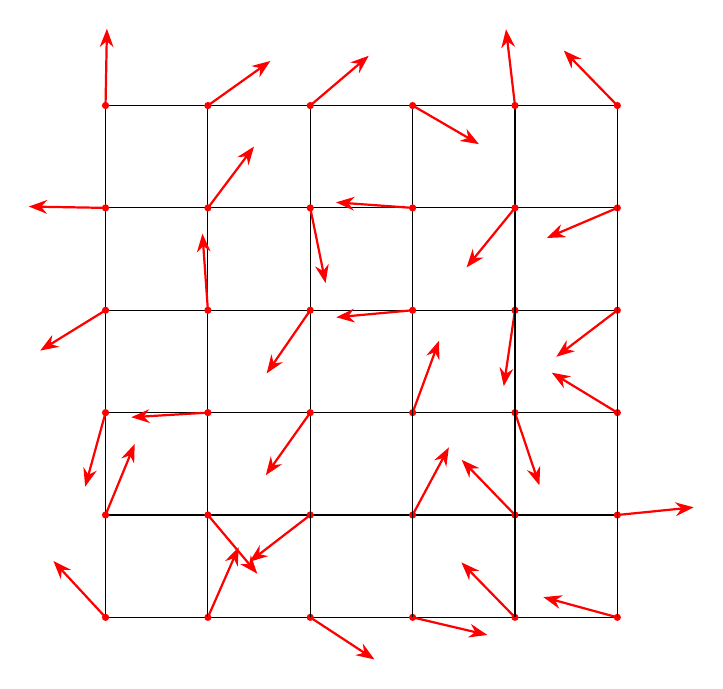
\begin{tikzpicture}[scale=0.65]
        \pgfmathsetseed{3432}
        \foreach \i in {0, 2, ..., 10} {
        \draw (\i, 0) -- (\i, 10);
        \draw (0, \i) -- (10, \i);
        \foreach \x in {0, 2, ..., 10} {
        \draw[-{Stealth}, red, thick] (\x,\i) -- ++(rnd*360:1.5);
        \fill[red] (\x,\i) circle (2pt);
        }
        }

    \end{tikzpicture}
    \caption{A zaj rácsának szemléltetése.}
\end{wrapfigure}
A Perlin-zaj egy úgynevezett gradiens-zaj. Eszerint rácspontokat határozunk
meg, amikhez egy véletlenszerű vektort rendelünk. A gradiens tábla ezeket a
véletlenszerű vektorokat tárolja. A vektorok dimenziószáma megegyezik a zaj
dimenziószámával. (Kétdimenziós zaj $\rightarrow$ kétdimenziós vektor)
\newpage
\subsubsection{Vektorgenerálás}
\begin{wrapfigure}[5]{r}{0.4\textwidth}
    \centering
    \vspace{-40pt}
    \hspace*{1.2cm}
    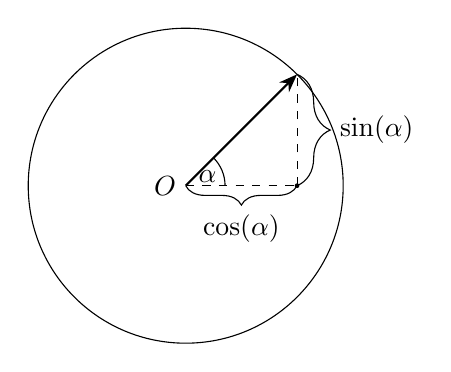
\begin{tikzpicture}[scale=2]
        \coordinate (O) at (0,0);
        \draw (O) circle (1cm);
        \pgfmathsetmacro{\angle}{45}
        \pgfmathsetmacro{\x}{cos(\angle)}
        \pgfmathsetmacro{\y}{sin(\angle)}
        \fill[black] (\x,0) circle (0.15mm);
        \draw[-{Stealth}, black, thick] (O) -- (\x, \y);
        \coordinate (A) at (\x, \y);
        \coordinate (B) at (\x, 0);
        \draw pic ["$\alpha$", draw=black, angle radius=5mm] {angle = B--O--A};
        \draw[dashed] (O) -- (B);
        \draw[decorate, decoration={brace, mirror, amplitude=7pt}]
        (O) -- (B) node[midway, below=7pt] {$\cos(\alpha)$};
        \draw[dashed] (B) -- (A);
        \draw[decorate, decoration={brace, mirror, amplitude=12pt}]
        (B) -- (A) node[midway, right=12pt] {$\sin(\alpha)$};

        \node[left] at (O) {$O$};
    \end{tikzpicture}
    \caption{A vektorok előállításának szemléltetése.}
\end{wrapfigure}
Generálunk egy véletlenszerű számot $[0;2\pi[$ intervallumban. Majd egyszerű
trigonometriával a szöget egy vektorrá alakítjuk, ahol a vektor $x$ komponense
a véletlen szög koszinusza, és az $y$ komponense a szög szinusza.
\vspace{2cm}
\subsection{Permutációs tábla}
A permutációs tábla kezdetben $0$-tól $255$-ig tartalmazza a számokat növekvő
sorrendben. Ezt a listát egy véletlenszám-generátor segítségével összekeverjük
és önmaga után fűzzük (ezzel egy $512$ elemű tömböt kapunk). Így a hashelésnél
elkerülhető a túlindexelés, ami gyorsítja a zajgenerálást, mivel elhagyható a
túlindexelésre való ellenőrzés. \\
\begin{algorithm}[H]
    \caption{Permutációs tábla létrehozása}
    \DontPrintSemicolon
    \Konstansok{MaxP=$512$}
    \Tipus{VéletlenSzámGenerátor=Osztály (\\
        \setlength\parindent{24pt} jelenlegiSzám:Egész\\
        \setlength\parindent{24pt} \textbf{Függvény} Következő:Egész\\
        )}

    \Eljaras{PermutaciosTablaGeneral (\textbf{Változó}: PermutaciosTabla:Tömb($1$..MaxP:Egész), \\
        Rand:VéletlenSzámGenerátor
        )}{
        % Változók
        \Valtozok{$i$, $j$, temp:Egész}
        ~\\
        \Ciklus{$i \coloneqq 1$-től $256$-ig}{
            PermutaciosTabla[$i$] $\coloneqq$ i
        }
        ~\\
        \Ciklus{$i \coloneqq 256$-tól $2$-ig $-1$-esével}{
            j $\coloneqq$ Rand.Következő() Mod ($i + 1$)  \\
            temp $\coloneqq$ PermutaciosTabla[$i$] \\
            PermutaciosTabla[$i$] $\coloneqq$ PermutaciosTabla[$j$] \\
            PermutaciosTabla[$j$] $\coloneqq$ temp \\
        }
        ~\\
        \Ciklus{$i \coloneqq 1$-től $256$-ig}{
            PermutaciosTabla[$i + 256$] $\coloneqq$ PermutaciosTabla[$i$]
        }
    }
\end{algorithm}
\newpage
\section{Zajszámítás}
\subsection{Rácspontok meghatározása}
\begin{wrapfigure}{r}{0.6\textwidth}
    \centering
    \vspace{-40pt}
    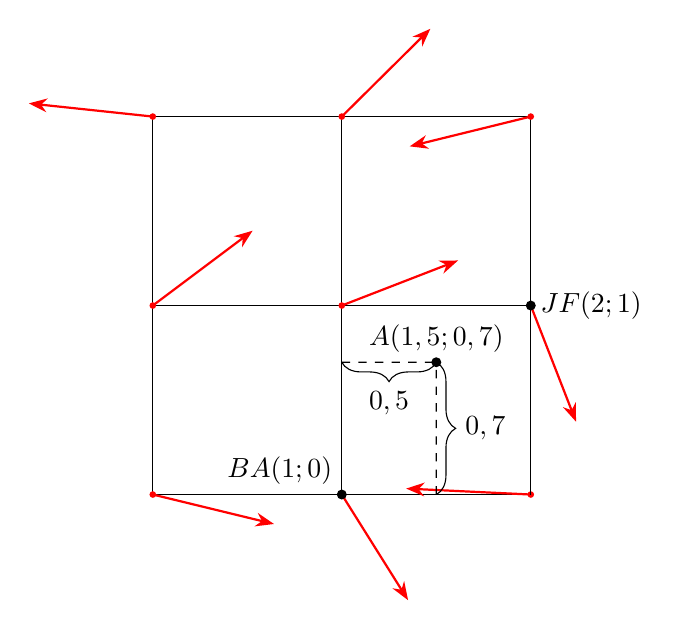
\begin{tikzpicture}[scale=0.6]
        \pgfmathsetseed{10}
        \pgfmathsetmacro{\racsok}{8}
        \pgfmathsetmacro{\racsokSzama}{2}
        \pgfmathsetmacro{\meret}{4}
        \foreach \i in {0, \meret, ..., \racsok} {
        \draw (\i, 0) -- (\i, \racsok);
        \draw (0, \i) -- (\racsok, \i);
        \foreach \x in {0, \meret, ..., \racsok} {
        \draw[-{Stealth}, red, thick] (\x,\i) -- ++(rnd*360:{\meret*0.66});
        \fill[red] (\x,\i) circle (2pt);
        }
        }

        \coordinate (A) at ({\meret + \meret * 0.5}, {\meret * 0.7});
        \fill (A) circle (3pt);
        \node[above] at (A) {$A(1,5;0,7)$};
        \coordinate (B) at (\meret, 0.0);
        \fill (B) circle (3pt);
        \node[above left] at (B) {$BA(1;0)$};
        \coordinate (C) at ({\meret * 2}, \meret);
        \fill (C) circle (3pt);
        \node[right] at (C) {$JF(2;1)$};

        \draw[dashed] (\meret, {\meret * 0.7}) -- (A);
        \draw[decorate, decoration={brace, mirror, amplitude=7pt}]
        (\meret, {\meret * 0.7}) -- (A) node[midway, below=7pt] {$0,5$};
        \draw[dashed] ({\meret + \meret * 0.5}, 0.0) -- (A);
        \draw[decorate, decoration={brace, mirror, amplitude=7pt}]
        ({\meret + \meret * 0.5}, 0.0) -- (A) node[midway, right=7pt] {$0,7$};
    \end{tikzpicture}
    \\
    \caption{A rácspont koordinátáinak szemléltetése.}
    \vspace{10pt}
\end{wrapfigure}
Először meghatározzuk, hogy az adott ($x$, $y$) pont melyik négyzetbe tartozik
ezt a bitenkénti ÉS $255$ művelettel tesszük, így az eredmény a $[0;255]$
tartományba fog esni: ha az érték nagyobb, mint $255$, akkor visszafordul az
intervallum elejére (pl. $256$-ból $0$ lesz). Ezt elvégezve az $x$-re és $y$-ra
megkapjuk a bal alsó rácspont koordinátáit. A bal alsó rácspont
koordinátáihoz hozzáadva $1$-et majd egy bitenkénti ÉS $255$ művelettel
megkapjuk a jobb felső rácspont koordinátáit. A négyzeten belüli pontot úgy
kapjuk meg, hogy a szám egész részét elhagyjuk. \\ \\
Pszeudókódban megvalósítva:
\begin{algorithm}
    \caption{Rácspontok és négyzeten belüli koordináták kiszámolása}

    \Tipus{Rácspont=Rekord (\\
        \setlength\parindent{24pt} balAlsóPontX, balAlsóPontY:Egész\\
        \setlength\parindent{24pt} jobbFelsőPontX, jobbFelsőPontY:Egész\\
        \setlength\parindent{24pt} relatívX, relatívY :Valós\\
        )}
    \Fuggveny{RacspontKiszamolasa(\textbf{Konstans}: $x$, $y$: Valós) : Rácspont}{
        \Valtozok{jelenlegiRácspont: Rácspont}
        jelenlegiRácspont.balAlsóPontX $\coloneqq$ ((Egész)floor($x$)) \& $256$ + $1$ \\
        jelenlegiRácspont.balAlsóPontY $\coloneqq$ ((Egész)floor($y$)) \& $256$ + $1$ \\
        ~\\
        jelenlegiRácspont.jobbFelsőPontX $\coloneqq$ (jelenlegiRácspont.balAlsóPontX
        $+ 1$) \& $256$ \\ jelenlegiRácspont.jobbFelsőPontY $\coloneqq$
        (jelenlegiRácspont.balAlsóPontY $+ 1$) \& $256$ \\
        ~\\
        jelenlegiRácspont.relatívX $\coloneqq x -$ floor($x$) \\
        jelenlegiRácspont.relatívY $\coloneqq y -$ floor($y$)
        ~\\
        \textbf{RacspontKiszamolasa} $\coloneqq$ jelenlegiRácspont
    }
\end{algorithm}
\subsection{Skaláris szorzat kiszámítása}
\subsubsection{Gradiens vektorok kiválasztása}
A gradiens vektorokat a permutációs tábla segítségével választjuk ki. Vesszük a
permutációs tábla $x$-edik elemét, hozzáadjuk az $y$ értékét, majd az így
kapott összeget használjuk indexként a permutációs táblában. Az így kapott
eredmény lesz az indexe a gradiens vektornak a gradiens táblából.
\begin{algorithm}
    \caption{Gradiens vektor kiválasztása}
    \Tipus{Vektor=Rekord (\\
        \setlength\parindent{24pt} x:Valós\\
        \setlength\parindent{24pt} y:Valós\\
        )}
    \Konstansok{MaxP=$512$, MaxG=$256$}
    \Valtozok{PermutaciosTabla:Tömb($1$..MaxP:Egész)}
    \Valtozok{GradiensTabla:Tömb($1$..MaxG:Egész)\\~\\}

    \Fuggveny{Hash(\textbf{Konstans}: $x$, $y$: Egész) : Egész}{
        \textbf{Hash} $\coloneqq$ PermutaciosTabla[PermutaciosTabla[$x$] + $y$]
    }
    ~\\
    \Fuggveny{GradiensVektorKivalaszt(\textbf{Konstans}: $x$, $y$: Egész) : Vektor}{
        \textbf{GradiensVektorKivalaszt} $\coloneqq$ GradiensTabla[hash($x$, $y$)]
    }
\end{algorithm}
\subsubsection{A sarkokból a pontba mutató vektorok kiszámítása}
Legyen a négyzeten belüli $P$ pont relatív koordinátái $(x_{0}, y_{0})$, ahol
$x_{0}, y_{0} \in [0;1]$. A rácsnégyzet sarkai legyen $A, B, C, D$.\\ Így a
sarkokból a pontba mutató vektorok:

\noindent
\begin{minipage}[t]{0.5\textwidth}
    \vspace{0pt}
    \begin{itemize}[noitemsep, leftmargin=*]
        \item \textbf{Bal alsó:} \tabto{3cm} $\vec{v}_{AP}(x_{0}, y_{0})$
        \item \textbf{Jobb alsó:} \tabto{3cm} $\vec{v}_{BP}(x_{0}-1, y_{0})$
        \item \textbf{Bal felső:} \tabto{3cm} $\vec{v}_{CP}(x_{0}, y_{0}-1)$
        \item \textbf{Jobb felső:} \tabto{3cm} $\vec{v}_{DP}(x_{0}-1, y_{0}-1)$
    \end{itemize}
\end{minipage}
\begin{minipage}[t]{0.5\textwidth}
    \vspace{0pt}
    \centering
    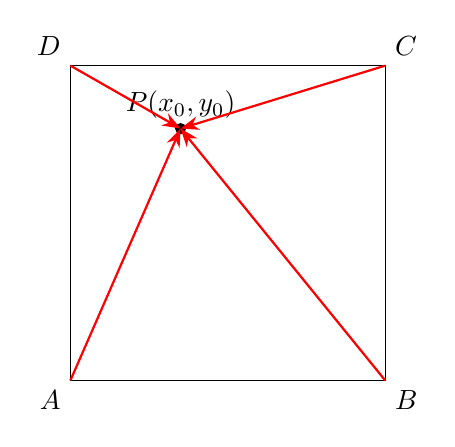
\begin{tikzpicture}
        \pgfmathsetseed{3432}
        \pgfmathsetmacro{\meret}{4}
        \coordinate (A) at (0, 0);
        \node[below left] at (A) {$A$};
        \coordinate (B) at (\meret, 0);
        \node[below right] at (B) {$B$};
        \coordinate (C) at (\meret, \meret);
        \node[above right] at (C) {$C$};
        \coordinate (D) at (0, \meret);
        \node[above left] at (D) {$D$};
        \draw (A) -- (B) -- (C) -- (D) -- cycle;

        \coordinate (P) at (1.4, 3.2);
        \fill (P) circle (2pt);
        \node[above] at (P) {$P (x_{0}, y_{0})$};
        \draw[-{Stealth}, red, thick] (A) -- (P);
        \draw[-{Stealth}, red, thick] (B) -- (P);
        \draw[-{Stealth}, red, thick] (C) -- (P);
        \draw[-{Stealth}, red, thick] (D) -- (P);

    \end{tikzpicture}
    \captionof{figure}{Relatív vektorok.}
\end{minipage}
\newpage
\subsubsection{Skaláris szorzat kiszámítása}
A vektorok meghatározása után kiszámítjuk az adott sarokhoz tartozó gradiens-
és relatív vektorok skaláris szorzatát. A skaláris szorzatot a matematikai
definíció alapján végezzük: $\vec{a} \cdot \vec{b} = x_{a}x_{b} + y_{a}y_{b} $
\begin{algorithm}
    \caption{Skaláris szorzat}
    \Tipus{Vektor=Rekord (\\
        \setlength\parindent{24pt} x:Valós\\
        \setlength\parindent{24pt} y:Valós\\
        )}

    \Fuggveny{SkalarisSzorzat(\textbf{Konstans}: $v1$, $v2$: Vektor) : Valós}{
        \textbf{SkalarisSzorzat} $\coloneqq$ v1.x * v2.x + v1.y * v2.y
    }
\end{algorithm}
\subsection{Interpoláció}
A kapott skalárszorzatokat végül egy simítófüggvény segítségével interpoláljuk
a tengelyek mentén.
\subsubsection{Simítófüggvény}
Simítófüggvényként a Ken Perlin által 2002-ben, az `Improved Noise'-ban
bevezetett függvényt hasznájuk. \cite{10.1145/566654.566636}
\[
    s(t) = 6t^{5} - 15t^{4} + 10t^{3}
\]
A függvény fontos jellemzője, hogy az első deriváltja és második deriváltja is
egyenlő 0-val $t=0$ és $t=1$ esetén is, így sima, folyamatos átmenet lesz a
rácsnégyzetetek közt.\\
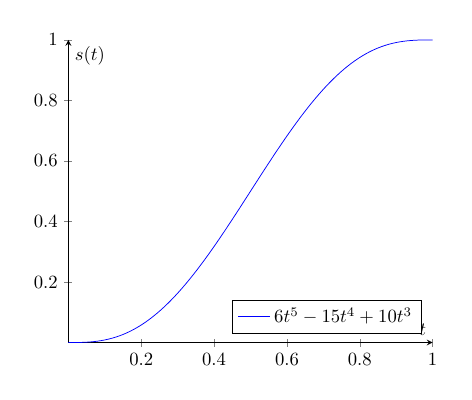
\begin{tikzpicture}[scale=0.675]
    \begin{axis}[
            axis lines = middle,
            xlabel = $t$,
            ylabel = {$s(t)$},
            legend pos = south east
        ]
        \addplot [
            domain=0:1,
            samples=100,
            color=blue,
        ] {6*x^5 - 15*x^4 + 10*x^3};
        \addlegendentry{$6t^{5} - 15t^{4} + 10t^{3}$}
    \end{axis}
\end{tikzpicture}
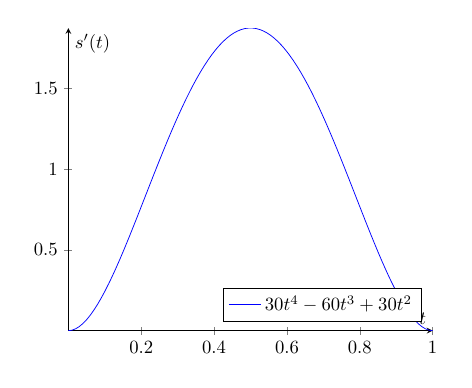
\begin{tikzpicture}[scale=0.675]
    \begin{axis}[
            axis lines = middle,
            xlabel = $t$,
            ylabel = {$s'(t)$},
            legend pos = south east
        ]
        \addplot [
            domain=0:1,
            samples=100,
            color=blue,
        ] {30*x^4 - 60*x^3 + 30*x^2};
        \addlegendentry{$30t^{4} - 60t^{3} + 30t^{2}$}
    \end{axis}
\end{tikzpicture}
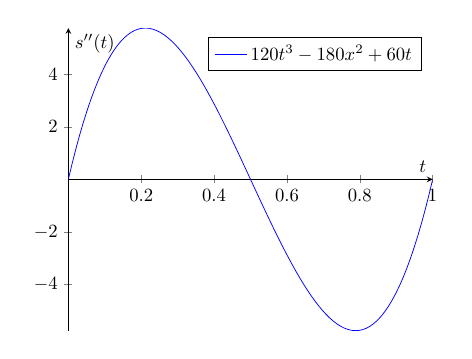
\begin{tikzpicture}[scale=0.675]
    \begin{axis}[
            axis lines = middle,
            xlabel = $t$,
            ylabel = {$s''(t)$},
            legend pos = north east
        ]
        \addplot [
            domain=0:1,
            samples=100,
            color=blue,
        ] {120*x^3 - 180*x^2 + 60*x};
        \addlegendentry{$120t^{3} - 180x^{2} + 60t$}
    \end{axis}
\end{tikzpicture}
\begin{algorithm}
    \caption{Simítófüggvény}
    \Fuggveny{Simitofuggveny(\textbf{Konstans}: t: Valós) : Valós}{
        \textbf{Simitofuggveny} $\coloneqq$ $6t^{5} - 15t^{4} + 10t^{3}$
    }
\end{algorithm}
\subsubsection{Interpoláció}
A végeredményt a skaláris szorzatok interpolálásával kapjuk. Kétdimenzió esetén
először kiszámoljuk a relatív x-koordináta simítófüggvénybeli értékét, majd
eszerint interpoláljuk a skaláris szorzatokat az x tengely mentén, tehát a
felső skaláris szorzatokat és az alsó skaláris szorzatokat. Majd kiszámoljuk a
relatív y-koordináta simítófüggvénybeli értékét, és eszerint interpoláljuk az
előző kettő interpolált részeredményt.
\begin{algorithm}
    \caption{Interpoláció}
    \Fuggveny{Interpolacio(\textbf{Konstans}: a, b, t: Valós) : Valós}{
        \textbf{Interpolacio} $\coloneqq$ $a + t \times (b - a)$
    }
\end{algorithm}
\newpage
\section{Teljes zajfüggvény}
Először kiszámoljuk a vizsgált pontot tartalmazó rácsnégyzet koordinátáit és a
ponton belüli relatív helyzetét a \textit{RacspontKiszamolasa} függvénnyel. Ezt
követően lekérjük a négy sarokhoz tartozó vektorokat a
\textit{GradiensVektorKivalaszt} függvénnyel, majd kiszámítjuk a sarkokból a
pontba mutató távolságvektorokat. Végül kiszámoljuk a skaláris szorzatukat az
adott sarkokhoz való vektoroknak a \textit{SkalarisSzorzat} segítségével. Végül
interpoláljuk a skaláris szorzatokat az \textit{Interpolacio} függvénnyel.
\begin{algorithm}
    \linespread{0.925}\selectfont
    \caption{Teljes zajfüggvény}
    \Tipus{Vektor=Rekord (x, y: Valós)}
    \Tipus{Rácspont=Rekord (\\
        \setlength\parindent{24pt} balAlsóPontX, balAlsóPontY:Egész\\
        \setlength\parindent{24pt} jobbFelsőPontX, jobbFelsőPontY:Egész\\
        \setlength\parindent{24pt} relatívX, relatívY:Valós\\
        )}

    \Fuggveny{Zaj(\textbf{Konstans}: $x$, $y$: Valós) : Valós}{
        \Valtozok{rácspont: Rácspont}
        \Valtozok{g00, g10, g01, g11: Vektor}
        \Valtozok{p00, p10, p01, p11: Vektor}
        \Valtozok{u, v, a, b: Valós}
        \Komment{1. Rácspont és relatív koordináták kiszámítása}
        rácspont $\coloneqq$ RacspontKiszamolasa($x$, $y$)\\
        \Komment{2. Gradiens vektorok lekérdezése}
        g00 $\coloneqq$ GradiensVektorKivalaszt(rácspont.balAlsóPontX, rácspont.balAlsóPontY)\\
        g10 $\coloneqq$ GradiensVektorKivalaszt(rácspont.jobbFelsőPontX, rácspont.balAlsóPontY)\\
        g01 $\coloneqq$ GradiensVektorKivalaszt(rácspont.balAlsóPontX, rácspont.jobbFelsőPontY)\\
        g11 $\coloneqq$ GradiensVektorKivalaszt(rácspont.jobbFelsőPontX, rácspont.jobbFelsőPontY)\\
        \Komment{3. Relatív vektorok definiálása}
        p00.x $\coloneqq$ rácspont.relatívX\\
        p00.y $\coloneqq$ rácspont.relatívY\\
        p10.x $\coloneqq$ rácspont.relatívX - $1.0$\\
        p10.y $\coloneqq$ rácspont.relatívY\\
        p01.x $\coloneqq$ rácspont.relatívX\\
        p01.y $\coloneqq$ rácspont.relatívY - $1.0$\\
        p11.x $\coloneqq$ rácspont.relatívX - $1.0$\\
        p11.y $\coloneqq$ rácspont.relatívY - $1.0$\\
        \Komment{4. Simítófüggvény alkalmazása}
        u $\coloneqq$ Simitofuggveny(rácspont.relatívX)\\
        v $\coloneqq$ Simitofuggveny(rácspont.relatívY)\\
        \Komment{5. Skaláris szorzatok kiszámítása és interpolálásuk}
        a $\coloneqq$ Interpolacio(SkalarisSzorzat(g00, p00), SkalarisSzorzat(g10, p10), u)\\
        b $\coloneqq$ Interpolacio(SkalarisSzorzat(g01, p01), SkalarisSzorzat(g11, p11), u)\\
        \textbf{Zaj} $\coloneqq$ Interpolacio(a, b, v)
    }
\end{algorithm}
\section{\textbf{F}ractal \textbf{B}rownian \textbf{M}otion (Fraktál zaj)} WIP \newpage
\printbibliography[heading=bibintoc,title={Forrásjegyzék}]
\end{document}